
\documentclass{article}
\usepackage{tikz}
\usetikzlibrary{positioning}
\title{Detailed Interview Summary Report}
\author{Generated by GPT Wrapper}
\date{\today}
\begin{document}
\maketitle

\section{Candidate Overview}
Sure! Here are the extracted pieces of information from the interview transcript:

1. **Candidate Name:** Alex Thompson
2. **Position Applied For:** Google STEP internship
3. **Interview Date:** Not explicitly mentioned in the transcript
4. **Technical Skills:** AI, computer vision, dynamic programming, optimization
5. **Problem-Solving Skills:** Creative problem-solving, debugging, adapting to constraints
6. **Communication Skills:** Articulate in explaining technical concepts
7. **Key Projects Discussed:** Frax AI (AI platform for analyzing X-rays and detecting fractures)
8. **Strengths:** Resourcefulness, technical knowledge, ability to explain complex concepts
9. **Areas for Improvement:** Consideration of potential collisions in URL shortening service design
10. **Final Recommendations:** Not explicitly stated in the transcript

If you have any specific questions or need further assistance, feel free to ask!

\section{Interview Summary}
The interview evaluated the candidate across multiple dimensions:
- **Technical Proficiency**: Sure! Here are the extracted pieces of information from the interview transcript:

1. **Candidate Name:** Alex Thompson
2. **Position Applied For:** Google STEP internship
3. **Interview Date:** Not explicitly mentioned in the transcript
4. **Technical Skills:** AI, computer vision, dynamic programming, optimization
5. **Problem-Solving Skills:** Creative problem-solving, debugging, adapting to constraints
6. **Communication Skills:** Articulate in explaining technical concepts
7. **Key Projects Discussed:** Frax AI (AI platform for analyzing X-rays and detecting fractures)
8. **Strengths:** Resourcefulness, technical knowledge, ability to explain complex concepts
9. **Areas for Improvement:** Consideration of potential collisions in URL shortening service design
10. **Final Recommendations:** Not explicitly stated in the transcript

If you have any specific questions or need further assistance, feel free to ask!
- **Problem-Solving Skills**: Sure! Here are the extracted pieces of information from the interview transcript:

1. **Candidate Name:** Alex Thompson
2. **Position Applied For:** Google STEP internship
3. **Interview Date:** Not explicitly mentioned in the transcript
4. **Technical Skills:** AI, computer vision, dynamic programming, optimization
5. **Problem-Solving Skills:** Creative problem-solving, debugging, adapting to constraints
6. **Communication Skills:** Articulate in explaining technical concepts
7. **Key Projects Discussed:** Frax AI (AI platform for analyzing X-rays and detecting fractures)
8. **Strengths:** Resourcefulness, technical knowledge, ability to explain complex concepts
9. **Areas for Improvement:** Consideration of potential collisions in URL shortening service design
10. **Final Recommendations:** Not explicitly stated in the transcript

If you have any specific questions or need further assistance, feel free to ask!
- **Communication**: Sure! Here are the extracted pieces of information from the interview transcript:

1. **Candidate Name:** Alex Thompson
2. **Position Applied For:** Google STEP internship
3. **Interview Date:** Not explicitly mentioned in the transcript
4. **Technical Skills:** AI, computer vision, dynamic programming, optimization
5. **Problem-Solving Skills:** Creative problem-solving, debugging, adapting to constraints
6. **Communication Skills:** Articulate in explaining technical concepts
7. **Key Projects Discussed:** Frax AI (AI platform for analyzing X-rays and detecting fractures)
8. **Strengths:** Resourcefulness, technical knowledge, ability to explain complex concepts
9. **Areas for Improvement:** Consideration of potential collisions in URL shortening service design
10. **Final Recommendations:** Not explicitly stated in the transcript

If you have any specific questions or need further assistance, feel free to ask!

\section{Strengths and Areas for Improvement}
Sure! Here are the extracted pieces of information from the interview transcript:

1. **Candidate Name:** Alex Thompson
2. **Position Applied For:** Google STEP internship
3. **Interview Date:** Not explicitly mentioned in the transcript
4. **Technical Skills:** AI, computer vision, dynamic programming, optimization
5. **Problem-Solving Skills:** Creative problem-solving, debugging, adapting to constraints
6. **Communication Skills:** Articulate in explaining technical concepts
7. **Key Projects Discussed:** Frax AI (AI platform for analyzing X-rays and detecting fractures)
8. **Strengths:** Resourcefulness, technical knowledge, ability to explain complex concepts
9. **Areas for Improvement:** Consideration of potential collisions in URL shortening service design
10. **Final Recommendations:** Not explicitly stated in the transcript

If you have any specific questions or need further assistance, feel free to ask!

\section{Graphical Representation}
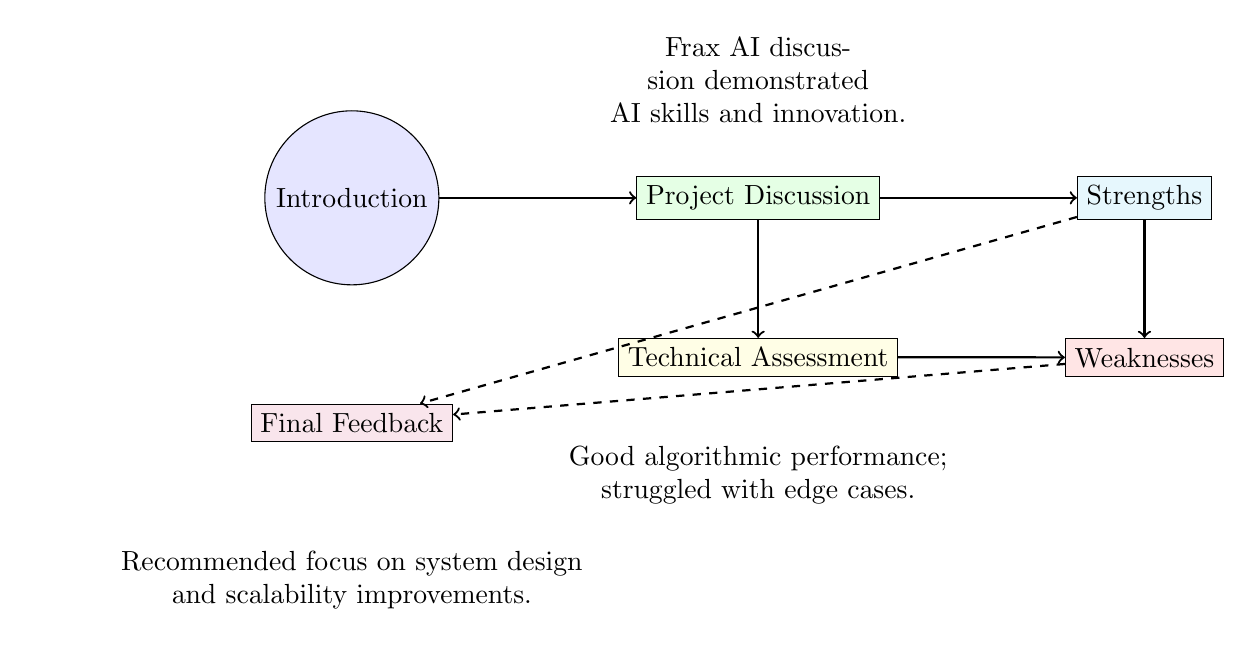
\begin{tikzpicture}
% Define nodes
\node[draw, circle, fill=blue!10] (intro) {Introduction};
\node[draw, rectangle, right=2.5cm of intro, fill=green!10] (projects) {Project Discussion};
\node[draw, rectangle, below=1.5cm of projects, fill=yellow!10] (technical) {Technical Assessment};
\node[draw, rectangle, right=2.5cm of projects, fill=cyan!10] (strengths) {Strengths};
\node[draw, rectangle, below=1.5cm of strengths, fill=red!10] (weaknesses) {Weaknesses};
\node[draw, rectangle, below=1.5cm of intro, fill=purple!10] (feedback) {Final Feedback};

% Draw arrows
\draw[->, thick] (intro) -- (projects);
\draw[->, thick] (projects) -- (technical);
\draw[->, thick] (projects) -- (strengths);
\draw[->, thick] (technical) -- (weaknesses);
\draw[->, thick] (strengths) -- (weaknesses);
\draw[->, thick, dashed] (weaknesses) -- (feedback);
\draw[->, thick, dashed] (strengths) -- (feedback);

% Add annotations
\node[above of=projects, yshift=0.5cm, text width=5cm, align=center] 
{Frax AI discussion demonstrated \\ AI skills and innovation.};
\node[below of=technical, yshift=-0.5cm, text width=5cm, align=center] 
{Good algorithmic performance; \\ struggled with edge cases.};
\node[below of=feedback, yshift=-1cm, text width=8cm, align=center] 
{Recommended focus on system design \\ and scalability improvements.};

\end{tikzpicture}

\section{Final Recommendations}
Sure! Here are the extracted pieces of information from the interview transcript:

1. **Candidate Name:** Alex Thompson
2. **Position Applied For:** Google STEP internship
3. **Interview Date:** Not explicitly mentioned in the transcript
4. **Technical Skills:** AI, computer vision, dynamic programming, optimization
5. **Problem-Solving Skills:** Creative problem-solving, debugging, adapting to constraints
6. **Communication Skills:** Articulate in explaining technical concepts
7. **Key Projects Discussed:** Frax AI (AI platform for analyzing X-rays and detecting fractures)
8. **Strengths:** Resourcefulness, technical knowledge, ability to explain complex concepts
9. **Areas for Improvement:** Consideration of potential collisions in URL shortening service design
10. **Final Recommendations:** Not explicitly stated in the transcript

If you have any specific questions or need further assistance, feel free to ask!

\end{document}
